% ============================================================================
% EnerTEF Journal Paper — Part 1: Front matter through System Architecture
% Target: IEEE Transactions on Smart Grid / Applied Energy / Energy and AI
% ============================================================================
\documentclass[journal]{IEEEtran}

\usepackage[utf8]{inputenc}
\usepackage[T1]{fontenc}
\usepackage{amsmath,amssymb,amsfonts}
\usepackage{algorithmic}
\usepackage{algorithm}
\usepackage{graphicx}
\usepackage{textcomp}
\usepackage{xcolor}
\usepackage{booktabs}
\usepackage{multirow}
\usepackage{hyperref}
\hypersetup{hidelinks}
\usepackage{cite}
\usepackage{bm}
\usepackage{subcaption}
\usepackage{tikz}
\usetikzlibrary{arrows.meta, positioning, shapes.geometric, fit, backgrounds, calc, decorations.pathreplacing}

\newcommand{\loss}{\mathcal{L}}
\newcommand{\fisher}{\mathbf{F}}
\newcommand{\params}{\bm{\theta}}
\newcommand{\paramsstar}{\bm{\theta}^{*}}
\newcommand{\ewclambda}{\lambda}
\newcommand{\real}{\mathbb{R}}

\begin{document}

\title{Closed-Loop Continual Learning for EV Charging:\\
From Autonomous Adaptation to Measured Savings}

\author{
\IEEEauthorblockN{
Abdelhaq Dabaghia\IEEEauthorrefmark{1}\IEEEauthorrefmark{2}
and Pedro Rodriguez\IEEEauthorrefmark{1}\IEEEauthorrefmark{2}
}
\IEEEauthorblockA{
\IEEEauthorrefmark{1}
Luxembourg Institute of Science and Technology (LIST)\\
L-4362 Esch-sur-Alzette, Luxembourg\\
Email: abdelhaq.dabaghia@list.lu, pedro.rodriguez@list.lu
}
\IEEEauthorblockA{
\IEEEauthorrefmark{2}
Department of Engineering, University of Luxembourg\\
L-4365 Esch-sur-Alzette, Luxembourg
}
}

\maketitle

 \begin{abstract}
Artificial-intelligence models are increasingly deployed at commercial energy sites to support forecasting and autonomous decision-making across a wide range of applications. However, their predictive performance degrades over time as operating conditions evolve, seasonal patterns shift, charging infrastructure expands, and user behaviour changes---a phenomenon known as concept drift. Existing strategies remain insufficient for real-world operation: periodic full-history retraining is computationally expensive as the dataset grows, rolling-window retraining discards the seasonal knowledge encoded in older data, and na\"ive fine-tuning on recent data leads to catastrophic forgetting of previously learned operating regimes. Although continual learning (CL) has received significant academic attention, its transition from offline experiments to continuously operating cyber-physical energy systems remains largely unexplored. In particular, existing studies rarely address the complete engineering chain required for autonomous adaptation, including cloud deployment, model lifecycle management, validation mechanisms, integration with real-time controllers, data reliability, and long-term operation in a real energy environment.

This paper presents an autonomous continual-learning architecture deployed as an operational prototype at a commercial energy site in Luxembourg, integrating AI forecasting, cloud-based model adaptation, and real-time operational control. The framework consists of: (i) two forecasting models---a PV LSTM and an EV CNN-LSTM---adapted nightly through an EWC-inspired proximal regulariser that uses a Memory Aware Synapses (MAS)-style output-sensitivity importance estimator; (ii) a tolerance-gated promotion mechanism with fail-safe retention that deploys a candidate only if it does not regress beyond a 5\% margin on a recent holdout, bounding---but not eliminating---the risk of deploying a worse model; and (iii) a direct coupling between the continually updated forecasts and a convex Model Predictive Control (MPC) scheduler that optimises electric-vehicle charging decisions under real ENTSO-E day-ahead electricity prices.

Beyond the algorithmic application of continual learning, this work demonstrates the complete pathway from initial model training and cloud deployment to integration with real-time control infrastructure. We present the EWC-inspired objective together with its Bayesian motivation, while making explicit that the deployed importance estimator is a MAS-style output-sensitivity proxy rather than an empirical Fisher estimator, and present the corresponding convex MPC formulation. Using real Leneda smart-meter data from Luxembourg, a representative nightly cycle reduces PV forecast MAE by 21.83\% and EV demand forecast MAE by 67.87\% relative to the static production models, driving a convex MPC loop against real day-ahead prices. A controlled $12$-cycle, five-seed sequential experiment ($240$ adaptation jobs) further isolates retention from plasticity: measured by backward transfer on a fixed winter reference window, bounded experience replay resists seasonal forgetting whereas the output-sensitivity regulariser does not improve retention over na\"ive fine-tuning, a paired advantage that is consistent across all five seeds ($11.1$~kW mid-stream, $p{=}0.002$). The paper also reports practical engineering challenges---framework incompatibilities, model-conversion (ONNX export) failures, data-quality degradation, and data-provenance verification---that are largely absent from the continual-learning literature. The primary contribution is therefore an operational architecture and real-site case study for safely integrating continual learning into an autonomous forecasting and MPC-based energy-management pipeline, rather than a novel CL algorithm.

\end{abstract}

\begin{IEEEkeywords}
Continual learning, autonomous AI systems, output-sensitivity
regularisation, memory aware synapses, model predictive control,
electric vehicle charging, concept drift, commercial energy site
\end{IEEEkeywords}

% ============================================================================
\section{Introduction}
\label{sec:intro}

A forecaster deployed at a commercial energy site is one link in a loop.
Predictions of photovoltaic (PV) generation and electric-vehicle (EV) charging
demand feed an optimisation-based controller; the controller issues setpoints
that move real power; the resulting consumption is metered and billed; and that
measurement is the only evidence the loop produced anything. Most deployed
forecasters, however, are static---trained once and maintained without
adaptation---which is untenable where seasons turn, behaviour shifts and
charging infrastructure is added, so that the data distribution drifts away
from the one the model was fitted to~\cite{gama2014survey}. Continual
learning (CL) addresses that drift, and the trade-off it must manage is between
plasticity, adapting to new conditions, and stability, retaining regimes that
are rare but operationally
important~\cite{mccloskey1989catastrophic,french1999catastrophic}.

What is almost never closed is the loop itself. CL for energy forecasting is
evaluated on held-out error; controllers are evaluated on the savings their
optimiser expects; and the two are reported separately. Neither figure touches
a meter. A saving computed by subtracting an optimised cost from an unmanaged
one, with both terms evaluated on the \emph{forecast}, is produced identically
by a system working perfectly and by one whose setpoints never leave the
process, whose price feed has frozen, or whose forecaster is being served
features it was not trained on. We know this because we built such a system and
then instrumented it to find out.

This paper reports a \emph{closed-loop} continual-learning architecture
operating at a commercial site in Dudelange, Luxembourg, and measures every
arrow of the loop: nightly autonomous adaptation of a PV LSTM and an EV
CNN--LSTM, a validation gate that decides whether each candidate is promoted, a
convex model-predictive controller that turns the promoted forecasts into
charging setpoints under real ENTSO-E day-ahead prices, and a settlement path
that reconciles the resulting schedule against metered demand. Closing it
required measuring the parts of the system that had never been observed, and
what that measurement found is as much the contribution as the architecture.

Three results follow. \emph{First}, the gap between reported and delivered
economics is large: over $21$ days on real prices, planned savings average
$11.5\%$ of the bill and settled savings $6.0\%$. \emph{Second}, closing the
loop surfaced thirteen defects, all but one invisible to any alarm, which share
a structure --- a component unable to do its job answers plausibly instead of
refusing. \emph{Third}, on the learning side a $240$-job multi-seed study shows
the deployed proximal regulariser does not prevent seasonal forgetting while
bounded replay does, identifying coverage of the past input distribution rather
than parameter anchoring as the operative mechanism.

Our central contribution is therefore not a new CL algorithm but an operational
architecture in which adaptation is connected to decisions and to measured
outcomes, together with the measurement practices that connection turns out to
require:

\begin{enumerate}

    \item An \textbf{autonomous continual-learning pipeline for energy forecasting} that adapts PV LSTM and EV CNN-LSTM models nightly through an EWC-inspired, MAS-style output-sensitivity regulariser that limits parameter drift, requiring no human intervention under normal operation.

    \item A \textbf{tolerance-gated promotion mechanism with fail-safe retention}, enabling reliable model promotion by rejecting candidates that regress beyond a fixed tolerance on a recent holdout, rather than relying on post-deployment rollback.

    \item A \textbf{direct evaluation of the impact of continual learning on energy management decisions}, linking forecast adaptation with MPC-based EV charging optimisation under real day-ahead electricity prices from the ENTSO-E Transparency Platform.

    \item A \textbf{mathematical formulation of the regularised adaptation objective and its Bayesian motivation} for recurrent and convolutional forecasting architectures, making explicit that the deployed importance estimator is a MAS-style output-sensitivity proxy rather than an empirical Fisher estimator, together with the practical approximations required for computationally efficient deployment.

    \item A \textbf{candid account of production-engineering challenges} encountered during the implementation of a continual learning workflow, including model-conversion issues, framework-compatibility constraints, data-quality limitations, and data-provenance verification.

\end{enumerate}

The remainder of this paper is organised as follows. Section II reviews related work on energy forecasting, continual learning, and AI-based energy management systems. Section III presents the proposed continual learning architecture and mathematical formulation. Section IV describes the experimental setup and deployment environment. Section V discusses the obtained results and their implications for energy management. Finally, Section VI concludes the paper and presents future research directions.


% ============================================================================
\section{Related Work}
\label{sec:related}

\subsection{Forecasting and continual learning in energy}
Short-term PV and load forecasting is dominated by recurrent and hybrid
convolutional--recurrent models~\cite{hochreiter1997long}; attention-based
architectures~\cite{vaswani2017attention,lim2021temporal} improve long-horizon
accuracy at data and parameter costs unfavourable for a single site re-adapted
nightly. Across that literature the forecaster is assumed fixed after
deployment.

Continual learning addresses the stability--plasticity dilemma through three
families. Regularisation methods penalise movement of important parameters:
EWC~\cite{kirkpatrick2017overcoming} weights an $L_2$ anchor by the diagonal
Fisher information --- an imperfect curvature
proxy~\cite{kunstner2019limitations} --- while Memory Aware
Synapses~\cite{aljundi2018memory} measures output sensitivity without labels,
which is closer to common practical implementations, including ours, than is
usually acknowledged. Rehearsal methods store or synthesise past
data~\cite{lopezpaz2017gradient,chaudhry2019efficient,shin2017continual},
resisting forgetting at a storage cost; architectural methods isolate
task-specific capacity~\cite{rusu2016progressive}. A comparative study on
building-energy forecasting~\cite{li2024building} reports regularisation as the
best stability--plasticity compromise in this data regime, which is what
motivated the deployed choice --- and which
Section~\ref{sec:results_seeds} does not reproduce over a seasonal stream.
Coupling forecasts to a downstream optimiser connects to
decision-focused learning~\cite{ng2024cost,zenke2017continual}.

\subsection{What is not measured, and the gap}
\label{sec:gap}
Three omissions are near-universal and together they are this paper's target.
\emph{First}, energy-domain CL is evaluated offline: nightly adaptation,
automated validation, fail-safe promotion and deployment into a live service
are rarely demonstrated under real conditions. \emph{Second}, forecast quality
is reported in isolation from the controller's economic outcome, and where an
economic figure does appear it is a \emph{planned} one, computed on the forecast
with no meter in the arithmetic --- so it cannot distinguish a working system
from a broken one. \emph{Third}, production failure modes are seldom reported,
yet they are a primary barrier to adoption and, as
Section~\ref{sec:defects} shows, they are largely invisible to the metrics the
field does report. We close all three by connecting adaptation to decisions and
decisions to metered outcomes, and by reporting what that connection revealed.

\section{System Architecture}
\label{sec:architecture}

\subsection{Site Description}
\label{sec:site}

The system described in this paper is deployed at a commercial energy
site in Luxembourg. The site comprises a rooftop photovoltaic
installation, two electric vehicle charging groups, EMOB1 (four DC
fast chargers, 300~kW each) and EMOB2 (four DC chargers of 400~kW and
eight AC chargers of 22~kW) and a grid connection to the DE-LU
day-ahead electricity market. All telemetry is metered at 15-minute
resolution via a national smart-metering platform (Leneda). Being a
single prosumer site behind one grid connection, we describe it as a
commercial energy site rather than an energy community, since it lacks
the multi-member, shared-allocation, and governance features of the
latter.

\begin{figure*}[t]
\centering
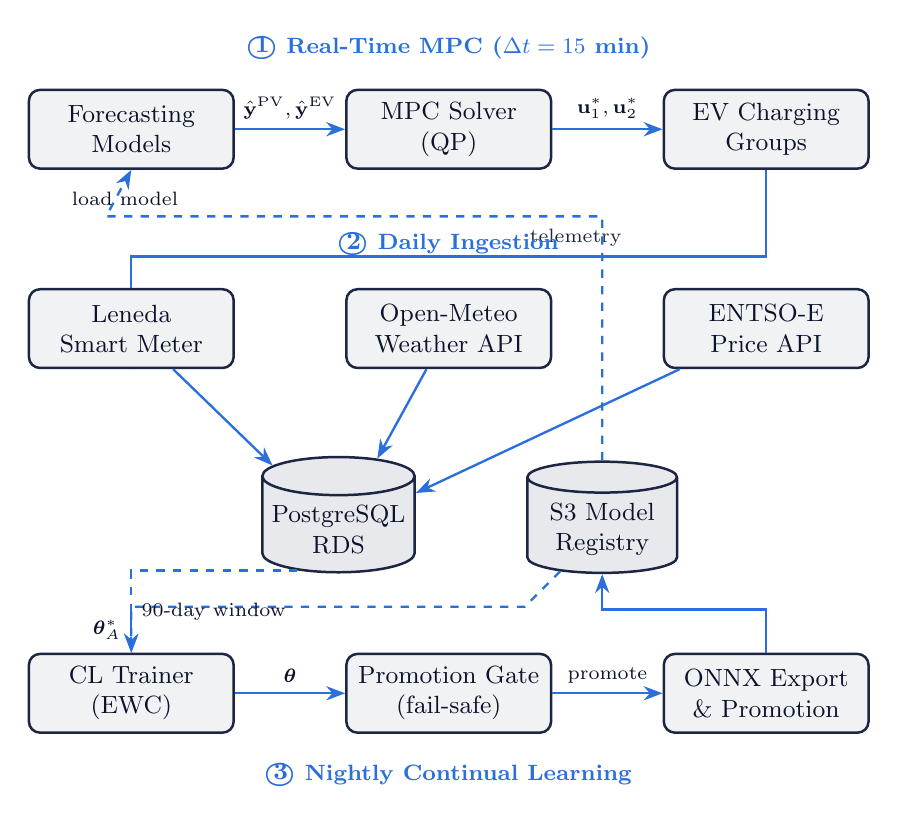
\begin{tikzpicture}[
    >=Stealth,
    node distance=0.9cm and 1.4cm,
]
\definecolor{navyDark}{HTML}{0B132B}
\definecolor{navyMed}{HTML}{1C2541}
\definecolor{skyAccent}{HTML}{2A6FDB}

\tikzset{
    component/.style={
        rectangle, rounded corners=4pt, draw=navyMed, line width=0.9pt,
        fill=navyMed!6, minimum height=1.0cm, minimum width=2.6cm,
        font=\small, align=center, text=navyDark,
    },
    datastore/.style={
        cylinder, shape border rotate=90, draw=navyMed, line width=0.9pt,
        fill=navyMed!10, minimum height=0.85cm, minimum width=1.9cm,
        font=\small, align=center, aspect=0.25, text=navyDark,
    },
    flow/.style={->, thick, draw=skyAccent, line width=0.85pt},
    looplabel/.style={font=\footnotesize\bfseries, color=skyAccent},
}

\node[component] (forecast) {Forecasting\\Models};
\node[component, right=of forecast] (mpc) {MPC Solver\\(QP)};
% MPC actuates only the two EV charging groups; the PV inverter is not a
% control variable in the formulation, so it is not shown as an actuator.
\node[component, right=of mpc] (hardware) {EV Charging\\Groups};

\node[component, below=1.5cm of forecast] (leneda) {Leneda\\Smart Meter};
\node[component, right=of leneda] (weather) {Open-Meteo\\Weather API};
\node[component, right=of weather] (entsoe) {ENTSO-E\\Price API};

\node[datastore, below=1.1cm of weather, xshift=-1.4cm] (postgres) {PostgreSQL\\RDS};
\node[datastore, right=1.4cm of postgres] (s3) {S3 Model\\Registry};

\node[component, below=3.6cm of leneda] (trainer) {CL Trainer\\(EWC)};
\node[component, right=of trainer] (validator) {Promotion Gate\\(fail-safe)};
\node[component, right=of validator] (exporter) {ONNX Export\\\& Promotion};

\draw[flow] (forecast) -- node[above, font=\scriptsize, text=navyDark]
    {$\hat{\mathbf{y}}^{\mathrm{PV}}, \hat{\mathbf{y}}^{\mathrm{EV}}$} (mpc);
\draw[flow] (mpc) -- node[above, font=\scriptsize, text=navyDark]
    {$\mathbf{u}_1^*, \mathbf{u}_2^*$} (hardware);
\draw[flow, dashed] (s3.north) -- ++(0,3.1) -- ++(-6.3,0) --
    node[near end, below, font=\scriptsize, text=navyDark] {load model} (forecast.south);

\draw[flow] (leneda) -- (postgres);
\draw[flow] (weather) -- (postgres);
\draw[flow] (entsoe) -- (postgres);

% Telemetry from the physical assets is metered by Leneda (then stored in
% PostgreSQL), NOT connected to the ENTSO-E price block. Routed on the
% background layer as an arc from the EV groups to the Leneda meter.
\begin{scope}[on background layer]
\draw[flow] (hardware.south) -- ++(0,-1.1)
    -| node[pos=0.15, above, font=\scriptsize, text=navyMed] {telemetry}
    (leneda.south);
\end{scope}

\draw[flow] (exporter.north) -- ++(0,0.55) -| (s3.south);
\draw[flow] (trainer) -- node[above, font=\scriptsize, text=navyDark]
    {$\params$} (validator);
\draw[flow] (validator) -- node[above, font=\scriptsize, text=navyDark]
    {promote} (exporter);
\draw[flow, dashed] (s3.south west) -- ++(-0.45,-0.45) -|
    node[near end, left, font=\scriptsize, text=navyDark] {$\params_A^*$} (trainer.north);
\draw[flow, dashed] (postgres.south west) -- ++(-0.7,0) -|
    node[near end, right, font=\scriptsize, text=navyDark] {90-day window} (trainer.north);

\node[looplabel, above=0.25cm of mpc] {\textcircled{\small 1} Real-Time MPC ($\Delta t = 15$~min)};
\node[looplabel, above=0.29cm of weather] {\textcircled{\small 2} Daily Ingestion};
\node[looplabel, below=0.25cm of validator] {\textcircled{\small 3} Nightly Continual Learning};

\end{tikzpicture}
\caption{System architecture. Three asynchronous loops share a common
data layer (PostgreSQL) and model registry (S3). Loop~1 runs every
15~minutes, consuming forecasts to produce optimal EV charging
setpoints for the two EV groups. Loop~2 ingests external data daily;
telemetry from the physical assets is metered by Leneda and stored in
PostgreSQL. Loop~3 fine-tunes the forecasters nightly with the
EWC-inspired regulariser and promotes validated improvements through a
fail-safe gate.}
\label{fig:overview}
\end{figure*}

\subsection{Three-Loop Architecture}
\label{sec:loops}
Three asynchronous loops run at distinct time scales over a shared PostgreSQL
data layer and an S3 model registry (Fig.~\ref{fig:overview}). Their separation
is what makes the loop closable: each writes what the next reads, and every
hand-off is recorded.

\emph{Loop~1, real-time control, every $15$~min.} A containerised service
downloads the current models --- serialised in ONNX for framework-agnostic
inference --- queries the latest weather forecast and day-ahead price, solves
the MPC programme of Section~\ref{sec:mpc}, publishes setpoints over MQTT and
persists the plan, the resulting KPIs and the forecast horizon.

\emph{Loop~2, daily ingestion.} Smart-meter telemetry from the Luxembourg
national platform, Open-Meteo weather and ENTSO-E day-ahead prices are written
to the shared data layer once a day.

\emph{Loop~3, nightly continual learning.} A scheduled trigger launches two
parallel jobs, one per forecaster. Each downloads the model currently in
production, extracts the most recent $90$~days, adapts it under the
output-sensitivity regulariser of Section~\ref{sec:ewc}, validates the
candidate on a held-out $7$~days and, only if the gate of
Section~\ref{sec:validation_gate} passes, exports and promotes it --- writing to
the exact registry keys Loop~1 reads, so a promotion changes what the controller
serves on its next cycle with no redeployment. This loop is the paper's central
object, and Section~\ref{sec:results_deployment} reports the first scheduled
cycle in which it rejected one candidate and promoted the other.

\subsection{Dataset and Data Layer Organisation}
\label{sec:dataset}

Experiments use real smart-meter data from the Leneda platform. The
principal dataset spans 15-minute PV, EMOB1, and EMOB2 telemetry.
Data quality varies by year, reflecting the site's phased deployment:
photovoltaic installation and the EMOB2 charging group were
commissioned progressively, resulting in near-zero activity for these
assets in the earliest part of the historical record. To avoid
conflating genuine seasonal variation with this commissioning ramp,
all experiments reported in Section~\ref{sec:results} restrict training
and evaluation to the period in which all three assets report
continuously. EMOB2 first appears on 2024-09-10, with complete 15-minute
coverage from October~2024 and a steady mean active load of 12--13~kW from
November~2024 onward; experiments therefore use the period from
2024-09-10, during which all
three assets exhibit sustained activity (PV mean production 79--93~kW;
combined EV demand mean 25--43~kW). Weather variables (global
horizontal, direct normal, and diffuse horizontal irradiance, cloud
cover, temperature, wind speed) are sourced from the Open-Meteo Archive
API at the site coordinates; day-ahead electricity prices for the
DE-LU bidding zone are sourced from the ENTSO-E Transparency Platform.

This heterogeneous data is organised within a shared relational
database adopting a layered schema architecture comprising four
logical domains: \texttt{historical}, \texttt{contextual},
\texttt{operational}, and \texttt{planning}. The \texttt{historical}
schema stores the validated smart-meter measurements described above,
used for model training, continual adaptation, and benchmarking,
whereas \texttt{contextual} contains the exogenous weather and price
data. Real-time system states are maintained within the
\texttt{operational} schema, while MPC-generated schedules and
optimisation outputs are persisted in the \texttt{planning} schema.
This architectural separation establishes a clear boundary between
offline learning and online decision-making, ensuring data provenance,
reproducibility, and reliable model updates. By preventing the mixing
of validated historical observations with temporary operational or
planning data, the framework mitigates data leakage and preserves the
integrity of continual learning in production environments. Further
discussion of these deployment considerations is provided in
Section~\ref{sec:defects}.
% ============================================================================
\section{Continual Learning Framework}
\label{sec:clframework}

\subsection{Problem Statement}
\label{sec:problem}
At each nightly cycle $k$ the system holds parameters $\params_{k-1}$ serving
production and receives a window $\mathcal{D}_k$ of recent site data. It must
produce $\params_k$ that predicts the coming horizon well (plasticity) without
losing regimes seen earlier in the record (stability), and must decide
autonomously whether $\params_k$ is fit to serve. Writing $\loss$ for the
forecasting loss and $\mathcal{D}_{<k}$ for the earlier record, the adaptation
problem is to reduce $\loss(\params_k; \mathcal{D}_k)$ without inflating
$\loss(\params_k; \mathcal{D}_{<k})$, under the constraint that
$\mathcal{D}_{<k}$ is not available in full --- storing the whole record is
what periodic full-history retraining does, and its cost grows without bound.
Sections~\ref{sec:ewc} and~\ref{sec:baselines} give the two mechanisms we
compare for this, and Section~\ref{sec:results_seeds} measures them over a
seasonal stream.

\subsection{Forecasting Architectures}
\label{sec:architectures}
Both forecasters are one-step predictors over a lookback window, with a dense
head and a non-negativity projection on the output; the $96$-step, $24$-hour
MPC horizon comes from recursive rollout. The PV model is an LSTM ($64$ hidden
units) over a $24$-hour, $96$-step lookback of $11$ features --- PV power, six
weather variables and four cyclic time encodings --- trained with mean squared
error. The EV model prepends two 1-D convolutions (kernel $3$; $32$ and $64$
filters) to an LSTM over a $7$-day, $672$-step lookback of $21$ features, and
is trained with the Huber loss ($\delta = 0.5$), which is more robust to the
heavy-tailed distribution of charging power. Neither architecture is a
contribution of this paper: both are the models already in production, and they
are described here only so the adaptation results can be read against them.

Because the horizon is produced autoregressively, the one-step holdout error
reported in Section~\ref{sec:results_forecasting} is an optimistic proxy for
$24$-hour trajectory quality: rollout compounds error. In production a physical
clipping safeguard bounds the trajectory, without which we observed exponential
error growth over the horizon --- a defect recorded in
Table~\ref{tab:defects}.

\subsection{Output-Sensitivity Regularisation}
\label{sec:ewc}

Our regulariser is \emph{inspired by} the proximal view of Elastic
Weight Consolidation (EWC): after training on data $\mathcal{D}_A$, adaptation
to new data $\mathcal{D}_B$ is penalised for moving important parameters
away from the previous optimum $\params_A^*$, so the influence of
$\mathcal{D}_A$ is retained without storing its raw samples. Classical EWC
weights this penalty by the diagonal Fisher information; in deployment we
instead use a MAS-style output-sensitivity importance
(Section~\ref{sec:practical_fisher}), and therefore \emph{do not rely on
the Fisher/Bayesian interpretation for any quantitative claim}. We first
recall the Bayesian motivation that gives rise to the proximal penalty
form, then describe the importance estimator actually used.

\subsubsection{Where the proximal form comes from, and what we do not claim}
\label{sec:bayesian}
\label{sec:fisher}
The quadratic proximal penalty has a standard Bayesian reading: a Laplace
approximation of the posterior over $\params$ after $\mathcal{D}_A$ gives a
Gaussian centred at $\params_A^*$ whose precision is the Hessian of the
negative log-posterior, and under a well-specified likelihood at a mode that
Hessian is approximated by the Fisher information. Retaining only its diagonal
reduces storage from $O(n^2)$ to $O(n)$ --- decisive at $n = 78{,}337$ for the
EV model --- and yields the familiar per-parameter spring of
Eq.~\eqref{eq:ewc_loss}. That derivation motivates the \emph{form} of the penalty
and we adopt it on those grounds; we refer the reader to Kirkpatrick
\emph{et~al.}~\cite{kirkpatrick2017overcoming} and to the curvature analyses
of~\cite{kunstner2019limitations} for its full statement and its limits.

We deliberately do not build on it further, for three reasons that our own
measurements supply. \emph{First}, the estimator actually deployed is not the
Fisher: it differentiates a batch-averaged squared model output with the
labels discarded, which is the Memory Aware Synapses construction
\cite{aljundi2018memory} rather than an empirical Fisher, and the two coincide
only under assumptions this regression setting does not make. \emph{Second}, a
companion transfer study on the same architecture
\cite{dabaghia2026representation} finds the source and target
Fisher differ by $211\times$ in scale, and that once that scale is equalised
the Fisher's \emph{origin} has no measurable effect on either plasticity or
retention --- so the quantity's Bayesian pedigree is not what determines its
behaviour here. \emph{Third}, the multi-cycle results of
Section~\ref{sec:results_seeds} show the proximal penalty does not prevent
seasonal forgetting at all, while bounded replay does, which points to
coverage of the past input distribution rather than parameter anchoring as the
operative mechanism. Accordingly, no quantitative claim in this paper rests on
a Fisher or Bayesian interpretation, and the importance estimator is described
below on its own terms.

\subsubsection{Practical Importance Estimation}
\label{sec:practical_fisher}
The empirical Fisher commonly used in EWC approximates the diagonal
Fisher Information Matrix through a sample average of squared
per-example log-likelihood gradients:

\begin{equation}
    \hat{F}_{ii}^{\mathrm{emp}}
    =
    \frac{1}{M}
    \sum_{j=1}^{M}
    \left(
    \frac{\partial
    \log p(y_j \mid \mathbf{x}_j,\boldsymbol{\theta})}
    {\partial \theta_i}
    \right)^2 .
    \label{eq:empirical_fisher}
\end{equation}

However, directly computing this estimator requires evaluating
parameter gradients for individual samples, which becomes expensive for
large datasets and frequent model updates. In our production
implementation, we therefore employ a computationally efficient
gradient-based parameter importance proxy computed at the mini-batch
level. Instead of relying on per-sample log-likelihood gradients, the
importance of each parameter is estimated from the sensitivity of the
model output:

\begin{equation}
    \Omega_i
    =
    \frac{1}{B}
    \sum_{b=1}^{B}
    \left(
    \frac{\partial}{\partial \theta_i}
    \frac{1}{|\mathcal{B}_b|}
    \sum_{j\in\mathcal{B}_b}
    \hat{y}_{j}^{\,2}(\boldsymbol{\theta})
    \right)^2 ,
    \label{eq:importance_proxy}
\end{equation}

where $B$ denotes the number of mini-batches and $\mathcal{B}_b$ is the
set of samples contained in batch $b$. The proposed estimator is
therefore not the empirical Fisher itself, but rather an output
sensitivity-based importance measure. It is conceptually closer to the
parameter importance formulation adopted in Memory Aware Synapses
(MAS)~\cite{aljundi2018memory}, which estimates parameter relevance from
the sensitivity of the model output without requiring explicit target
labels.

Both empirical Fisher-based EWC and output sensitivity-based approaches
aim to identify parameters whose modification may significantly affect
previously acquired knowledge, although they capture different notions
of parameter importance. We adopt this batch-level estimator because it
provides a favourable computational trade-off for autonomous nightly
retraining, reducing the number of gradient evaluations from
sample-level computations to mini-batch updates while maintaining an
effective mechanism for limiting drift of the parameters most salient to
recent operating conditions. We note two honest caveats. First,
$\Omega_i$ is estimated on the \emph{same} 90-day window used for
adaptation, so the method protects parameters salient to \emph{recent}
conditions rather than a fixed historical memory; we therefore claim no
seasonal-knowledge preservation beyond what a rolling 90-day window can
provide. Second, because Eq.~\eqref{eq:importance_proxy} differentiates a
batch-averaged output and then squares, per-sample gradients may partly
cancel within a batch, so $\Omega_i$ is not equivalent to an average of
squared sample-level gradients; it is used as a lightweight importance
heuristic, not as a Fisher estimate.
\subsubsection{Regularisation Objective}
\label{sec:ewc_loss}

Classical EWC introduces the diagonal Fisher approximation of the
previous-task posterior into the Bayesian formulation and minimises the
resulting negative log-posterior. In our deployment we retain this
proximal quadratic form but substitute the MAS-style output-sensitivity
importance $\Omega_i$ of Eq.~\eqref{eq:importance_proxy} for the diagonal
Fisher, yielding the output-sensitivity regularisation (OSR) objective:

\begin{equation}
\mathcal{L}_{\mathrm{OSR}}(\params)
=
\mathcal{L}_{\mathrm{data}}(\params,\mathcal{D}_B)
+
\frac{\lambda}{2}
\sum_{i=1}^{n}
\Omega_{i}
(\theta_i-\theta_{A,i}^{*})^2 .
\label{eq:ewc_loss}
\end{equation}

where $\loss_{\mathrm{data}}$ is the forecasting loss of
Section~\ref{sec:architectures} --- mean squared error for PV, Huber
($\delta = 0.5$) for EV. The parameters
$\theta_{A,i}^{*}$ represent the previously learned model parameters,
while $\Omega_{i}$ denotes the estimated importance of parameter
$\theta_i$ obtained from the output-sensitivity estimator. Replacing the
Fisher by $\Omega_i$ is the only quantitative departure from classical
EWC; all subsequent claims rely on $\Omega_i$ rather than on the
Fisher/Bayesian interpretation.

The hyperparameter $\ewclambda$ controls the stability--plasticity
trade-off by regulating the strength of the constraint imposed on
previously learned parameters. In this deployment, $\ewclambda=1000$ was
selected empirically to balance adaptation to new operating conditions
with preservation of previously acquired forecasting behaviour.
\subsubsection{What the penalty does, and its limits}
The gradient of~\eqref{eq:ewc_loss} acts as a per-parameter spring of stiffness
$\ewclambda$ times the importance: where importance is near zero the parameter
adapts freely, and where it is large, deviation is penalised in proportion to
importance and drift. As $\ewclambda \to \infty$ the model freezes; as
$\ewclambda \to 0$ it reduces to naive fine-tuning. We set
$\ewclambda = 1000$. Section~\ref{sec:results_seeds} measures what this buys
over a seasonal stream, and the answer is nothing that bounded replay does not
buy more cheaply --- a result we report rather than an outcome the derivation
anticipates.

\subsubsection{Training Algorithm}

Algorithm~\ref{alg:ewc} summarises one output-sensitivity regularisation
cycle, executed nightly per forecasting model.

\begin{algorithm}[t]
\caption{Output-Sensitivity Regularisation Cycle (per model, nightly)}
\label{alg:ewc}
\begin{algorithmic}[1]
\REQUIRE Baseline $\params_A^*$, new data $\mathcal{D}_B$ (90~d),
holdout $\mathcal{D}_{\mathrm{hold}}$ (7~days), $M{=}500$,
$\ewclambda{=}1000$, learning rate $\eta$, epochs $E$, tolerance $\tau{=}1.05$
\STATE Download $\params_A^*$ and scalers from S3
\STATE Verify provenance (physical origin) of
$\mathcal{D}_B,\mathcal{D}_{\mathrm{hold}}$
\STATE Sample $M$ points from $\mathcal{D}_B$; compute $\Omega_i$
via Eq.~\eqref{eq:importance_proxy}
\STATE $\params \leftarrow \params_A^*$ \hfill (clone)
\FOR{$e = 1$ to $E$}
    \FOR{each mini-batch in $\mathcal{D}_B$}
        \STATE $\params \leftarrow \params - \eta \nabla_{\params}
        \loss_{\mathrm{OSR}}(\params)$ \hfill (Eq.~\eqref{eq:ewc_loss})
    \ENDFOR
\ENDFOR
\STATE $\mathrm{MAE}_{\mathrm{new}} \leftarrow \mathrm{eval}(\params, \mathcal{D}_{\mathrm{hold}})$
\STATE $\mathrm{MAE}_{\mathrm{base}} \leftarrow \mathrm{eval}(\params_A^*, \mathcal{D}_{\mathrm{hold}})$
\IF{$\mathrm{MAE}_{\mathrm{new}} \le \mathrm{MAE}_{\mathrm{base}} \times \tau$}
    \STATE Export $\params$ to ONNX; verify native/ONNX equivalence;
    atomic upload to S3 \algorithmicreturn{} \textsc{Promote}
\ELSE
    \STATE Retain $\params_A^*$ in production \algorithmicreturn{} \textsc{Reject}
\ENDIF
\end{algorithmic}
\end{algorithm}

% ============================================================================
\section{Autonomous Deployment Pipeline}
\label{sec:deployment}

We designed this autonomous
execution framework for Algorithm~\ref{alg:ewc}, where continual learning
cycles are performed without manual intervention while remaining subject
to automated validation and safety constraints. These mechanisms provide
controlled model evolution by preventing the deployment of degraded
updates and preserving the reliability of the operational forecasting
pipeline.
\subsection{Validation-Gated Promotion}
\label{sec:validation_gate}

To ensure reliable model evolution, each continual learning cycle
terminates with an automated validation gate before any update is
deployed. The newly adapted candidate model $\params$ is evaluated
against the currently deployed model $\params_A^*$ using an independent
holdout period $\mathcal{D}_{\mathrm{hold}}$, consisting of the most
recent days of observations .
The candidate model is promoted only if its forecasting performance
satisfies:

\begin{equation}
    \mathrm{MAE}(\params,\mathcal{D}_{\mathrm{hold}})
    \leq
    \tau \,
    \mathrm{MAE}(\params_A^*,\mathcal{D}_{\mathrm{hold}})
    \label{eq:validation}
\end{equation}

where $\tau=1.05$ introduces a 5\% tolerance margin to account for
natural variability in the holdout evaluation period while preventing
the deployment of significantly degraded models. This mechanism
provides a safeguard against erroneous adaptations and enables controlled
model updates in a continuously operating environment.

The validation process evaluates three complementary forecasting
metrics. The mean absolute error (MAE) measures the average magnitude of
prediction deviations, the root mean square error (RMSE) penalises larger
forecasting errors, and the normalised mean absolute error (NMAE)
provides a scale-independent performance indicator:

\begin{equation}
\begin{bmatrix}
\mathrm{MAE} \\[2mm]
\mathrm{RMSE} \\[2mm]
\mathrm{NMAE}
\end{bmatrix}
=
\begin{bmatrix}
\frac{1}{N_h}\sum_i |y_i-\hat{y}_i|
\\[4mm]
\sqrt{\frac{1}{N_h}\sum_i (y_i-\hat{y}_i)^2}
\\[4mm]
\frac{\mathrm{MAE}}
{\frac{1}{N_h}\sum_i |y_i|}
\end{bmatrix}
\label{eq:forecast_metrics}
\end{equation}

where $N_h=|\mathcal{D}_{\mathrm{hold}}|$ denotes the number of samples
within the validation horizon.




\paragraph{What the tolerance does and does not guarantee}
The $5\%$ margin accounts for holdout variability; it bounds but does not
eliminate the risk of promoting a degraded model, and it is a relative test
only --- a candidate is compared to its predecessor, never to a model-free
baseline. Section~\ref{sec:defects} records what that omission cost. For the EV
model the observed MAE differences exceed the estimated sampling uncertainty
(standard error about $3.1$~kW), though a rigorous assessment on this
autocorrelated series would require block bootstrap or HAC corrections.

\subsection{Fail-Safe Retention}

If validation fails, the candidate is rejected, $\params_A^*$ is retained
unchanged, the rejection is logged, and the system continues operating
with the previous model until the next cycle. This is \emph{fail-safe
promotion rejection} rather than post-deployment rollback: the pipeline
prevents an unsafe candidate from ever reaching production, as opposed to
deploying it, detecting degradation, and then restoring a prior version.
Dated backups of every previously promoted model are nonetheless retained
in the registry, so a manual restore to an earlier version remains
possible if needed. The worst-case outcome of a single cycle is therefore
promotion rejection (no change). This bounds, but does not eliminate, the
risk of deploying a worse model: an improvement on a 7-day holdout need
not persist in future operation, and the 5\% tolerance ($\tau=1.05$)
explicitly admits candidates up to 5\% worse than the incumbent.

% ============================================================================
\section{Model Predictive Control Integration}
\label{sec:mpcintegration}

\subsection{Model Predictive Control Formulation}
\label{sec:mpc}

The energy management layer employs a receding-horizon Model Predictive
Control (MPC) strategy to coordinate the charging flexibility of the two
EV charging groups while exploiting photovoltaic generation and
time-varying electricity prices. At each optimisation cycle, the
controller computes the charging adjustment vectors
$\mathbf{u}_1,\mathbf{u}_2\in\mathbb{R}^{H}$ over a prediction horizon
of length $H$. The controlled charging power is expressed as

\[
P_{\mathrm{EV}_j}^{\mathrm{ctrl}}(k)
=
P_{\mathrm{EV}_j}^{\mathrm{base}}(k)
+
u_j(k),
\]

where $P_{\mathrm{EV}_j}^{\mathrm{base}}$ denotes the forecasted
uncontrolled demand and $u_j(k)$ represents the optimisation decision.

The resulting grid power exchange is

\[
P_{\mathrm{grid}}(k)
=
P_{\mathrm{EV}_1}^{\mathrm{ctrl}}(k)
+
P_{\mathrm{EV}_2}^{\mathrm{ctrl}}(k)
-
P_{\mathrm{PV}}(k),
\]

which is decomposed into non-negative import and export variables to
account for electricity purchase and surplus photovoltaic injection.

The MPC optimisation problem is formulated as

\begin{equation}
\begin{aligned}
\min_{\mathbf{u}_1,\mathbf{u}_2}
\quad &
w_{\mathrm{imp}}
\sum_k
\pi_k
P_{\mathrm{imp}}(k)
\frac{\Delta t}{1000}
-
w_{\mathrm{exp}}
\sum_k
\pi_k
P_{\mathrm{exp}}(k)
\frac{\Delta t}{1000}
\\
&
+
w_u
\sum_{j=1}^{2}
\|\mathbf{u}_j\|_2^2
+
w_{\mathrm{ramp}}
\sum_{j=1}^{2}
\|\Delta\mathbf{u}_j\|_2^2
\end{aligned}
\label{eq:mpc_objective}
\end{equation}

subject to

\begin{align}
u_{\min}
&\le
u_j(k)
\le
u_{\max},
\\
P_{\mathrm{EV}_j}^{\min}
&\le
P_{\mathrm{EV}_j}^{\mathrm{ctrl}}(k)
\le
P_{\mathrm{EV}_j}^{\max},
\\
|u_j(k+1)-u_j(k)|
&\le
R_{\max},
\\
\sum_k u_j(k)
&=
0,
\\
P_{\mathrm{imp}}(k)-P_{\mathrm{exp}}(k)
&=
P_{\mathrm{grid}}(k),
\\
P_{\mathrm{imp}}(k),
P_{\mathrm{exp}}(k)
&\ge
0.
\end{align}

The objective simultaneously minimises electricity procurement costs,
maximises the utilisation of surplus photovoltaic energy, limits
unnecessary charging adjustments, and enforces smooth charging
trajectories. The energy-conservation constraint
($\sum_k u_j(k)=0$) ensures that the controller redistributes charging
demand over time without modifying the total energy delivered to the
vehicles. This aggregate per-group constraint is a deliberate
simplification relative to per-vehicle arrival, departure, and
state-of-charge constraints, adopted because the site exposes only
group-level setpoints; it may therefore shift demand within the horizon
in ways a per-vehicle model would forbid.

With the quadratic penalty weight $w_u>0$, the objective is strictly
convex in the control pair $(\mathbf{u}_1,\mathbf{u}_2)$ and the feasible
set is convex, so the problem is a convex quadratic programme with a
unique optimal \emph{control pair}; we claim uniqueness for the control
vectors only. The import/export variables share a single symmetric price
$\pi_k$ (Eq.~\eqref{eq:mpc_objective}), which omits network charges,
taxes, and retailer margins and is justified here by the site's direct
exposure to the wholesale DE-LU market; with strictly positive symmetric
prices, simultaneous import and export is precluded at the optimum, so
$P_{\mathrm{imp}},P_{\mathrm{exp}}$ are the positive and negative parts of
the net grid power (asymmetric tariffs extend this directly). The optimal
control actions depend continuously on the forecast inputs, making the
MPC particularly suitable for integration with the proposed continual
learning framework.

\subsection{The Forecast-to-Decision Gap}
\label{sec:forecast_decision_gap}

Let $\boldsymbol{\epsilon}=\hat{\mathbf{y}}-\mathbf{y}$ denote the
forecast error. The MPC cost suboptimality relative to a clairvoyant
controller, $\Delta C = C_{\mathrm{real}}(\mathbf{u}^*(\hat{\mathbf{y}}))
- C_{\mathrm{real}}(\mathbf{u}^*(\mathbf{y}))$, depends on the
\emph{interaction} between $\boldsymbol{\epsilon}$ and the price vector
$\boldsymbol{\pi}$, not on $\|\boldsymbol{\epsilon}\|$ alone: an error
during a low-price period has negligible economic consequence, while
the same-magnitude error during a price peak directly inflates realised
cost. This observation motivates evaluating continual learning by its
effect on \emph{realised MPC cost}, not forecast-accuracy metrics in
isolation (Section~\ref{sec:results_mpc}), and motivates two directions
for future work discussed in Section~\ref{sec:discussion}: cost-weighted
importance estimation, and decision-focused end-to-end training of the
forecaster through a differentiable representation of the MPC solver.

% ============================================================================
% ============================================================================
% v5 Section V -- the settlement methodology.
%
% This is the section Table~\ref{tab:defects} points at throughout. Without it
% the defect table is a list of anecdotes; with it, each row has a measurement
% behind it.
%
% Every figure here is from Data/results/e18_mpc_two_sites.csv (21 days, real
% ENTSO-E prices) or from the deployment record, and each is recomputed in the
% commit that introduced it.
% ============================================================================

\section{Settling a controller's economics}
\label{sec:settle}

A forecast-driven controller is almost always reported through one number: the
saving it expects to make. That number is produced by subtracting the cost of
an optimised schedule from the cost of an unmanaged one. The subtraction is
sound; what varies, and what is rarely stated, is which demand each term is
evaluated against.

We distinguish three quantities. They are computed from the same plan
$u^{\star}$ and differ only in what they are settled against, and the
differences between them are the subject of this section.

\subsection{Three quantities, one plan}

\paragraph{Planned savings.} The optimiser's own estimate: both the baseline
and the optimised cost are evaluated on the \emph{forecast} demand
$\hat{y}$. Nothing in the arithmetic touches a meter, and no property of the
physical site can change the result. A controller whose setpoints never leave
the process, whose price feed has frozen, or whose forecaster is served
features it was not trained on produces this number exactly as a working one
does.

\paragraph{Counterfactual savings.} The plan $u^{\star}$, decided on the
forecast, settled against the demand $y$ that actually arrived---but on a site
where that plan was never dispatched. This is an honest estimate of what the
controller would have banked, and it is what most offline evaluations
implicitly report. It is not a measurement of the site.

\paragraph{Settled savings.} The plan was dispatched, the setpoints were
accepted by the chargers, and the resulting consumption is settled against
metered demand and the day-ahead price that applied. This is the only one of
the three the site can bank.

The distinction is not pedantic. Over 21 days of the deployed configuration
under real ENTSO-E day-ahead prices, planned savings average
$+9.55$~EUR/day, or $11.5\%$ of the unmanaged bill. Settling the same plans
against metered demand gives $+7.86$~EUR/day on a larger realised bill:
$6.0\%$. The relative figure is thus overstated by nearly a factor of two,
and the absolute one by $1.69$~EUR/day.\footnote{The discrepancy in the
baseline itself---$82.89$ planned against $130.52$ settled---is the forecaster
under-predicting demand, and is the same defect quantified in
Table~\ref{tab:defects}.} Under the synthetic price curve the notebook
originally used, the same plans report $63.9\%$ planned against $38.6\%$
settled; price realism and settlement are independent sources of overstatement
and both apply.

\subsection{When the record can be trusted}
\label{sec:boundary}

Settlement requires knowing which setpoints were actually commanded. That is a
question about the control database, not about the controller, and the two
became answerable at different moments.

At this site the first successful publish to the chargers occurred at
\texttt{06:19:31~UTC}. From that instant the controller was acting on the
physical plant. But the database could not yet say so: the schema recorded one
status for the whole cycle rather than one per charger, so rows written before
\texttt{06:33:52~UTC}---when the revision carrying per-charger actuation
status was deployed---carry \texttt{pending} even for setpoints that were
dispatched and accepted.

Settlement therefore keys on \texttt{06:33:52}, not on \texttt{06:19:31}. The
later timestamp is not when control began; it is when the \emph{record} of
control became reliable, and that is the property a settlement query depends
on. Admitting the earlier window would settle genuinely dispatched steps as
$u=0$, understating the controller rather than overstating it---the safer
direction, but wrong, and wrong silently.

Both instants are retained and reported, because they answer different
questions. \texttt{06:19:31} is when the site began being controlled and is
the correct marker for any display of controller activity.
\texttt{06:33:52} is when settlement may begin. Conflating them, in either
direction, produces a figure that cannot be reproduced from the database.

\subsection{What settlement requires of the system}

Stating the three quantities is easy; producing the third is not. Settled
savings can only be computed where four things hold simultaneously, and each
was absent at this site at some point during the study:

\begin{enumerate}
\item \textbf{The setpoints reached the plant}, and the system recorded that
they did---rather than recording that they were computed.
\item \textbf{The price applied was the price billed.} A constant fallback
makes an energy-conserving shift worthless by construction, so a settled figure
computed over such a period is exactly zero regardless of the controller.
\item \textbf{The metered demand is present and fresh} for the settled period,
with any imputed value marked as imputed rather than returned as data.
\item \textbf{The settlement boundary is known}, as in
Section~\ref{sec:boundary}, so that the period settled is the period the
database can speak about.
\end{enumerate}

Each of these is a precondition that the reported-savings figure does not
have. That asymmetry is the practical argument of this paper: the number these
systems are judged by is the one that survives every failure, and the number
that would have caught those failures is the one nobody computes.

\subsection{Prospective protocol}

Because every settled figure in this paper is necessarily retrospective, and
because retrospective analysis of one's own deployment invites the objection
that the hypotheses were formed after the data was seen, the settlement window
reported in Section~\ref{sec:results} was pre-registered: the metrics, the
number of days, and the acceptance criterion were fixed and committed before
the first settleable day.\footnote{\texttt{PREREGISTRATION\_prospective.md} in
the accompanying repository, committed before the window opened.} The window
begins at the first cycle for which all four preconditions above hold
simultaneously, which at this site is \texttt{2026-09-22 06:04~UTC}---not the
date control began, and not the date the system was declared operational.


\section{Experimental Setup}
\label{sec:experimental}


\subsection{Models and Training Configuration}

Table~\ref{tab:hyperparams} summarises training hyperparameters for
both forecasting models, held constant across all reported experiments.

\begin{table}[t]
\centering
\caption{Training hyperparameters}
\label{tab:hyperparams}
\begin{tabular}{@{}lcc@{}}
\toprule
\textbf{Parameter} & \textbf{PV LSTM} & \textbf{EV CNN-LSTM} \\
\midrule
Lookback $T$ & 96 (24~h) & 672 (7~days) \\
Sequential features $d_s$ & 11 & 21 \\
Next-step features $d_n$ & 10 & 20 \\
Training window & 90 days & 90 days \\
Holdout & 7 days & 7 days \\
Regularisation $\ewclambda$ & 1000 & 1000 \\
Importance samples $M$ & 500 & 500 \\
Data loss & MSE & Huber ($\delta{=}0.5$) \\
Validation tolerance $\tau$ & 1.05 & 1.05 \\
\bottomrule
\end{tabular}
\end{table}
\subsection{Baseline Methods}
\label{sec:baselines}

To assess the effectiveness of the proposed autonomous continual
learning framework, three forecasting strategies are considered.

\begin{itemize}
    \item \textbf{Static model}: the forecasting model is trained once
    and deployed without further adaptation. This represents the
    conventional deployment strategy adopted in many operational energy
    forecasting systems.

    \item \textbf{Na\"ive fine-tuning}: the production model is updated
    using newly available data without any mechanism to preserve
    previously acquired knowledge ($\ewclambda=0$). This baseline isolates
    the effect of continual adaptation alone and serves as a reference for
    evaluating catastrophic forgetting.

    \item \textbf{Output-sensitivity regulariser (OSR, proposed)}: the
    forecasting model is updated using the EWC-inspired objective defined
    in Eq.~\eqref{eq:ewc_loss}, where parameter updates are regularised
    according to their MAS-style output-sensitivity importance. This
    strategy aims to balance adaptation to evolving operating conditions
    with retention of previously learned forecasting behaviour.

    \item \textbf{Bounded experience replay}: a rehearsal baseline that
    keeps a fixed-capacity reservoir of $B{=}2000$ past raw samples
    (reservoir sampling~\cite{lopezpaz2017gradient}), chained across cycles,
    and mixes it into each cycle's current window before optimisation
    ($\ewclambda{=}0$). Unlike OSR, it stores a bounded amount of raw data;
    we include it to test whether constraining \emph{data coverage} rather
    than \emph{parameters} better resists forgetting.

    \item \textbf{Replay${+}$OSR}: bounded experience replay combined with the
    output-sensitivity penalty ($\ewclambda{=}1000$), to test whether the two
    mechanisms are complementary.
\end{itemize}



\section{Results}
\label{sec:results}
We report the loop arrow by arrow: forecasting accuracy under a single
adaptation cycle (Section~\ref{sec:results_forecasting}); the regulariser
against naive fine-tuning on an identical window
(Section~\ref{sec:results_controlled}); retention over a $12$-cycle seasonal
stream, the study that separates the mechanisms
(Section~\ref{sec:results_seeds}); the pipeline's autonomous behaviour, including
a gate decision observed in production
(Section~\ref{sec:results_deployment}); and the controller's economics, planned
and settled (Section~\ref{sec:results_mpc}). Unless stated otherwise
$\ewclambda = 1000$, $M = 500$ importance samples and a promotion tolerance of
$1.05$ apply throughout, these being the deployed values.

\subsection{Forecasting Accuracy}
\label{sec:results_forecasting}

The forecasting performance of the proposed autonomous continual
learning framework was evaluated on an independent 7-day holdout period
following a representative nightly adaptation cycle for each model,
executed on the AWS SageMaker infrastructure described in
Section~\ref{sec:architecture}. Each cycle uses a 90-day training window
and a disjoint 7-day holdout immediately following it.
Table~\ref{tab:ev_results} summarises the validation results for both
forecasting models.

\begin{table}[t]
\centering
\caption{Validation results on the 7-day holdout (real Leneda data;
representative cycle).}
\label{tab:ev_results}
\begin{tabular}{@{}lcc@{}}
\toprule
\textbf{Model} & \textbf{MAE (kW)} & \textbf{Improvement} \\
\midrule
\multicolumn{3}{@{}l}{\textit{PV LSTM}} \\
\quad Static production model & 47.24 & --- \\
\quad Adapted (output-sensitivity) & 36.93 & \textbf{21.83\%} \\
\midrule
\multicolumn{3}{@{}l}{\textit{EV CNN-LSTM}} \\
\quad Static production model & 42.04 & --- \\
\quad Adapted (fine-tuning) & 13.51 & \textbf{67.87\%} \\
\bottomrule
\end{tabular}
\end{table}














Compared with the static production models, adaptation substantially
improves forecasting accuracy. The PV MAE falls from 47.24~kW to
36.93~kW (21.83\%), and the EV MAE from 42.04~kW to 13.51~kW (67.87\%);
for the EV model the RMSE (73.53$\rightarrow$22.19~kW) and NMAE
(0.975$\rightarrow$0.321) improve consistently, indicating that the gain
is not an artefact of a single metric.

The EV improvement exceeds that of PV, consistent with greater concept
drift in EV demand. A caveat applies to the EV figure, and it is not the
one about commissioning that an earlier draft of this work stated. The
static baseline was fitted from 2024-09-10 to 2025-10-20 ($38{,}883$
steps), with the final $90$~days held out. That window \emph{begins} on
the day EMOB2 first reports, so the baseline is not a pre-commissioning
model: the commissioning ramp (10~September--31~October~2024) covers about
$13\%$ of it and the remaining eleven months are steady-state operation of
both chargers. What the figure may still conflate is growth in EV demand
\emph{after} the baseline's cut-off with the value of continual adaptation
itself. Separating the two requires a baseline retrained on an equally
recent but frozen window, which we leave as future work. The EV candidate promoted in this cycle was a na\"ive
nightly fine-tune, whereas the PV adaptation used the output-sensitivity
regulariser; the controlled comparison of
Section~\ref{sec:results_controlled} isolates the regulariser from
na\"ive fine-tuning on an identical window.

Importantly, both adapted models satisfy the tolerance-gated promotion
criterion introduced in Section~\ref{sec:validation_gate}, allowing them
to be deployed automatically without manual intervention. These results
demonstrate that the proposed framework can improve forecasting
performance while maintaining the safety requirements necessary for
autonomous production deployment.

Figure~\ref{fig:ewc_curves} illustrates the optimisation dynamics during
the eight-epoch regularised fine-tuning cycle. The Huber forecasting loss
decreases steadily from 0.00859 to 0.00356, while the regularisation
term simultaneously decreases from 0.00129 to 0.00037. Rather than
indicating a conflict between adaptation and knowledge preservation,
this behaviour suggests that the optimiser converges towards a new
solution that improves prediction accuracy while remaining close to the
previously deployed parameter configuration in the parameter directions
identified as important by the adopted importance estimator. This
empirical behaviour is consistent with the stability--plasticity
objective underlying continual learning.

\begin{figure}[t]
\centering
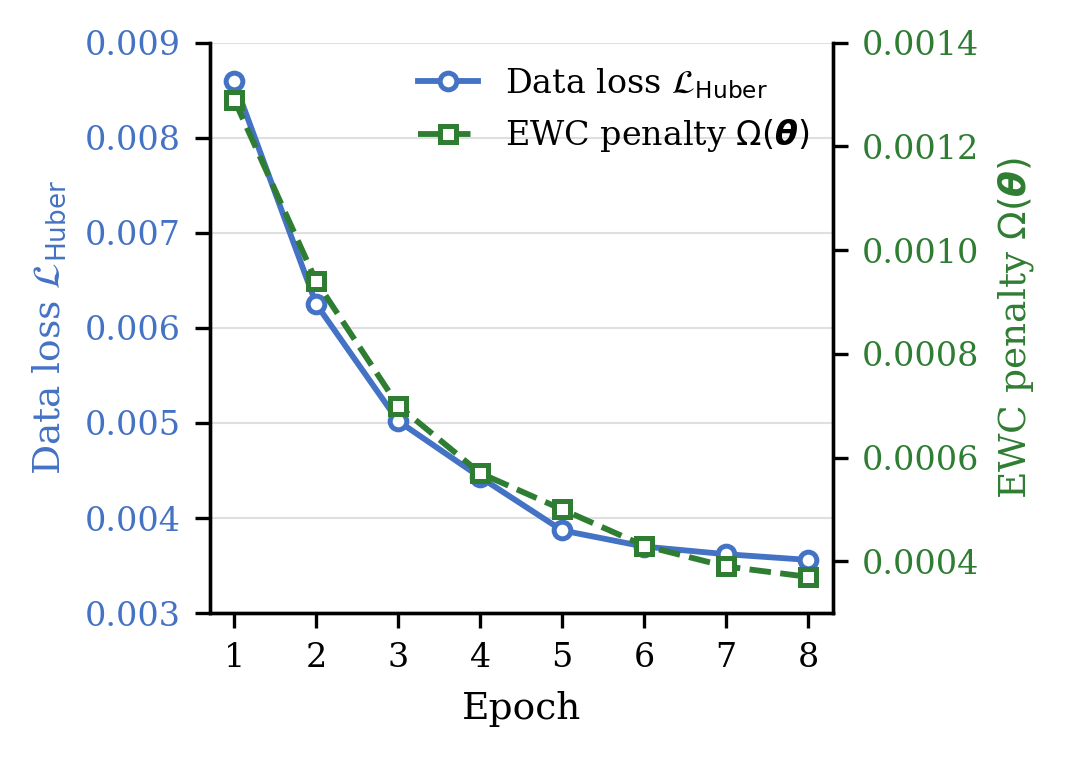
\includegraphics[width=\columnwidth]{ewc_training_curves.png}
\caption{Training dynamics of the proposed output-sensitivity adaptation
during a representative eight-epoch continual learning cycle. Both the
forecasting loss and the parameter regularisation term decrease
throughout optimisation, indicating successful adaptation while
preserving previously acquired knowledge.}
\label{fig:ewc_curves}
\end{figure}
%%%%%%%%%%%%%%%%%%%%%%%%%%%%%%%%%%%%%%%%%%%%%%%%%%%%%%%%%%%%%%%%%%%%%%%%%%%
\subsection{Regularised versus Na\"ive Adaptation}
\label{sec:results_controlled}

The holdout comparison of Section~\ref{sec:results_forecasting} contrasts
an adapted model against a frozen static baseline, and therefore
measures the combined effect of \emph{using recent data} and \emph{the
regularisation strategy}. To isolate the contribution of the
output-sensitivity regulariser itself, we ran a controlled experiment on
the PV model in which the training window, holdout, initialisation, and
optimiser were held fixed, and only the regularisation coefficient
$\lambda$ was varied. Three configurations were compared: the frozen
static model; na\"ive fine-tuning ($\lambda=0$, no regularisation); and
the proposed output-sensitivity regulariser ($\lambda=1000$).
Table~\ref{tab:controlled} reports the resulting holdout MAE.

\begin{table}[t]
\centering
\caption{Controlled PV comparison on an identical window: static
baseline, na\"ive fine-tuning, and the output-sensitivity regulariser.}
\label{tab:controlled}
\begin{tabular}{@{}lcc@{}}
\toprule
\textbf{Configuration} & \textbf{MAE (kW)} & \textbf{Improvement} \\
\midrule
Static production model & 47.24 & --- \\
Na\"ive fine-tune ($\lambda=0$) & 37.49 & 20.64\% \\
Output-sensitivity ($\lambda=1000$) & 36.93 & \textbf{21.83\%} \\
\bottomrule
\end{tabular}
\end{table}

Two observations follow. First, the majority of the improvement over the
static baseline (20.64 of 21.83 percentage points) is attributable to
retraining on recent data rather than to the regulariser: na\"ive
fine-tuning alone recovers most of the gain. Second, on this window the
regulariser yields a small additional accuracy improvement
(37.49$\rightarrow$36.93~kW) \emph{while} constraining the parameters it
estimates as important, so its principal role would be to protect previously
acquired behaviour at negligible cost to current-window accuracy rather
than to maximise single-cycle error reduction. We report this modest
effect transparently: on a single cycle the regulariser is not the main
driver of accuracy. Whether it actually protects earlier regimes over
repeated cycles cannot be judged here---this is a \emph{plasticity}
measurement on the recent window---and is settled by the controlled
multi-cycle study of Section~\ref{sec:results_seeds}.

\subsection{Multi-Cycle Sequential Retention: A Controlled Multi-Seed Study}
\label{sec:results_seeds}

The preceding comparisons are \emph{single-cycle} and measure plasticity
on the recent window; they cannot reveal catastrophic forgetting, which by
definition requires evaluating retained accuracy on an earlier regime after
adapting to later ones. We therefore ran a controlled sequential study that
is the central empirical validation of this paper. Starting from the same
frozen baseline, the PV~LSTM was adapted over a $12$-cycle stream that walks
from winter~2024 to winter~2025 in $+30$-day steps (each cycle uses a
$90$-day training window ending at that step). At every cycle we additionally
evaluate the model on a \emph{fixed} early-winter reference window
(1~Jan--19~Mar~2024) that the stream passed at cycle~0, so its error measures
retention of that regime. Four adaptation strategies were compared under
\emph{identical} windows and seeds---na\"ive ($\lambda{=}0$), OSR
($\lambda{=}1000$), bounded experience replay, and Replay${+}$OSR
(Section~\ref{sec:baselines})---each replicated over five random seeds and
chained cycle-to-cycle (parameters, and the replay reservoir where
applicable), for $4\times5\times12=240$ SageMaker adaptation jobs. Retention
is quantified by backward transfer relative to the anchor,
$\mathrm{BWT}(k)=\mathrm{MAE}_{\mathrm{ref}}(k)-\mathrm{MAE}_{\mathrm{ref}}(0)$,
where positive values denote forgetting (in the sense of
Lopez-Paz~\emph{et~al.}~\cite{lopezpaz2017gradient}).

\begin{figure}[t]
\centering
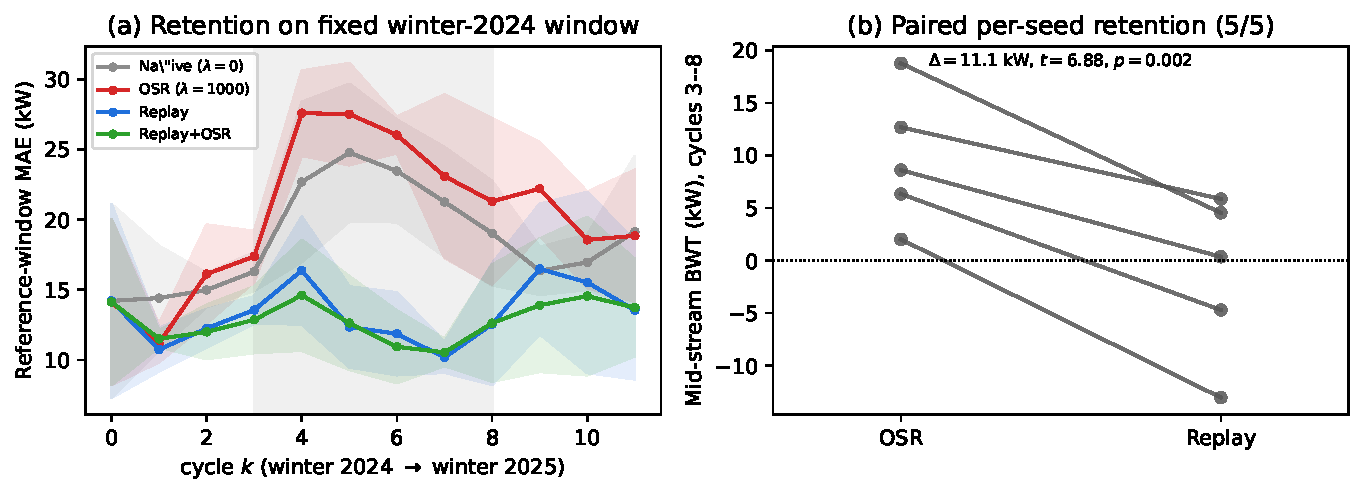
\includegraphics[width=\columnwidth]{bwt_seeds.pdf}
\caption{Multi-cycle retention (PV~LSTM, five seeds). (a)~Reference-window
MAE versus cycle (mean; shaded $\pm1$~s.d.\ over seeds): na\"ive and OSR
forget markedly in mid-stream (summer, cycles~3--8, shaded), whereas Replay
and Replay${+}$OSR stay flat. (b)~Per-seed mid-stream BWT for OSR versus
Replay; Replay retains better on \emph{all five} seeds.}
\label{fig:bwt_seeds}
\end{figure}

\begin{table}[t]
\centering
\caption{Multi-cycle retention and plasticity (PV~LSTM, mean$\pm$s.d.\ over
five seeds). BWT in kW; positive $=$ forgetting. Mid-stream is cycles~3--8
(furthest from the winter reference); plasticity is the recent-window MAE at
the final cycle.}
\label{tab:multicycle}
\begin{tabular}{@{}lccc@{}}
\toprule
\textbf{Strategy} & \textbf{BWT$_{\mathrm{mid}}$} & \textbf{BWT$_{\mathrm{peak}}$}
& \textbf{Plasticity} \\
& (kW) & (kW) & MAE (kW) \\
\midrule
Na\"ive ($\lambda{=}0$)      & $+7.04\pm7.18$ & $+13.07\pm8.52$ & $8.54$ \\
OSR ($\lambda{=}1000$)       & $+9.68\pm6.37$ & $+15.63\pm4.66$ & $9.37$ \\
Replay                        & $\mathbf{-1.39\pm7.70}$ & $\mathbf{6.83\pm6.94}$ & $13.82$ \\
Replay${+}$OSR                & $\mathbf{-1.77\pm6.64}$ & $\mathbf{5.67\pm5.41}$ & $13.04$ \\
\bottomrule
\end{tabular}
\end{table}

Three findings follow (Table~\ref{tab:multicycle}, Fig.~\ref{fig:bwt_seeds}).
\emph{First, bounded replay resists forgetting whereas OSR does not.} Replay
holds mid-stream BWT near zero ($-1.39$~kW) while na\"ive and OSR degrade
substantially ($+7.04$ and $+9.68$~kW). \emph{Second, and importantly, the
proposed OSR regulariser does not improve retention over na\"ive fine-tuning
in this setting}---its mid-stream BWT is if anything slightly larger
($+9.68$ vs.\ $+7.04$~kW; paired $t=-1.62$, $p=0.18$, not significant),
consistent with $\Omega$ being estimated on the same rolling $90$-day window
and thus protecting \emph{recent} rather than seasonally distant parameters
(Section~\ref{sec:fisher}). \emph{Third, the replay advantage is
statistically robust.} Comparing OSR and Replay on the same seeds, Replay
reduces mid-stream BWT by $11.07$~kW, with the same sign on all five seeds
(paired $t$-test $t=6.88$, $p=0.0023$; one-sided Wilcoxon signed-rank
$p=0.031$, its floor at $n{=}5$). The na\"ive-vs-Replay gap is likewise
consistent ($8.43$~kW, $5/5$ seeds, $p=0.0065$). We report both tests because
at $n{=}5$ the parametric test carries a normality assumption while the
non-parametric test cannot fall below $p=0.031$; the effect's significance
rests on their agreement and on the unanimous sign, not on any single test.

Two honest qualifications accompany these results. (i)~Retention is bought
with \emph{plasticity}: Replay's recent-window MAE at the final cycle is
higher ($13.8$ vs.\ $8.5$~kW for na\"ive), the expected stability--plasticity
trade-off. (ii)~The endpoint (cycle~11) understates forgetting because the
stream returns to winter and na\"ive/OSR mechanically recover on the
reference; the effect is therefore reported at its mid-stream and peak, where
the regimes are most dissimilar. Finally, that adding OSR to Replay changes
neither retention nor the ranking (Replay${+}$OSR $\approx$ Replay) indicates
that, once data coverage of the earlier regime is maintained, the proximal
weight penalty contributes little---pointing to \emph{coverage of the past
input distribution}, rather than parameter anchoring, as the operative
mechanism.

The same verdict is reached independently, and by a different route, in a
companion study of \emph{cross-site} transfer
\cite{dabaghia2026representation}: there the shift is geographic rather than
seasonal, the target is an independent published trial rather than the site's
own past, and yet no regulariser variant---including a true empirical Fisher
and an EWC${+}$replay hybrid---beats a warm-start fine-tune with a small
replay buffer. We regard the agreement of two settings that share only the
architecture as stronger evidence than either result alone, and we note the
overlap explicitly so it is not mistaken for a single finding reported twice.
The two studies are complementary rather than redundant: the companion work
cannot observe seasonal forgetting, because a single transfer step has no
stream, and the present study cannot observe the representation effect that
dominates its cross-site transfers. A parameter-space diagnostic supports this reading: across all
four strategies the cumulative weight drift $\lVert\params_k-\params_0\rVert$
grows at essentially the same rate, yet retention diverges sharply, so
weight-space proximity does not govern retention here. We note that this shift
is \emph{seasonal} within a single site, that $n{=}5$ seeds is modest (the
paired design is what confers power), and that a geographic multi-site
evaluation remains future work.
%%%%%%%%%%%%%%%%%%%%%%%%%%%%%%%%%%%%%%%%%%%%%%%%%%%%%%%%%%%%%%%%%%%%%%%%%%%
\subsection{Autonomous Deployment Reliability}
\label{sec:results_deployment}

Achieving improved forecasting accuracy represents only one aspect of
an autonomous continual learning system. In operational energy
management, the greater challenge lies in ensuring that model
adaptation, validation, and deployment can be executed without human
intervention while guaranteeing that software failures never compromise
the forecasting service. Consequently, the robustness of the deployment
pipeline becomes as important as the learning algorithm itself.

\paragraph{The gate rejecting a candidate, observed.}
Until 2026-09-24 every candidate that reached the export stage had
satisfied~\eqref{eq:validation}, so the gate could be described but not
shown to decide. On that date the first \emph{scheduled} autonomous cycle
--- launched by a daily rule rather than by hand --- produced opposite
verdicts for the two models within the same run:

\begin{center}
\footnotesize
\begin{tabular}{@{}lcccl@{}}
\toprule
\textbf{Model} & \textbf{Incumbent} & \textbf{Candidate} &
\textbf{Threshold} & \textbf{Verdict} \\
& MAE (kW) & MAE (kW) & $1.05\times$ & \\
\midrule
PV LSTM      & $34.91$ & $38.32$ & $36.66$ & REJECT \\
EV CNN--LSTM & $27.17$ & $13.37$ & --- & PROMOTE \\
\bottomrule
\end{tabular}
\end{center}

\noindent The PV candidate regressed by $9.75\%$, exceeding the $5\%$
tolerance, and was refused; the incumbent continued to serve forecasts
without interruption. The EV candidate improved by $50.80\%$ and was
promoted, advancing the model served to the MPC without human
intervention. The improvement's size is itself informative and should not
be read as the value of continual adaptation: the incumbent it replaced
was $29$~days old, so much of the gain measures the cost of \emph{being
stale} rather than the benefit of the regulariser.

\paragraph{Failures after successful optimisation.}
Across the retraining campaigns the framework also encountered deployment
failures occurring after successful model optimisation. In multiple
adaptation cycles the candidate models satisfied the validation-gated
promotion criterion and were therefore eligible for production deployment,
yet the subsequent ONNX export stage failed because of toolchain-specific
limitations associated with shape inference and recurrent neural network
serialisation. These failures originated entirely from the deployment
infrastructure rather than the continual learning algorithm, illustrating
the practical complexity of translating research models into
production-ready AI services.

The proposed architecture explicitly separates the learning,
validation, export, model registry, and deployment stages of the MLOps
pipeline. This separation enables fault isolation, preventing failures
within one stage from propagating to the remainder of the autonomous
workflow. Whenever ONNX export failed, the validated checkpoint was
preserved while deployment was automatically aborted, allowing the
previous production model to continue serving forecasts without service
interruption. As a result, autonomous adaptation remained operational
despite repeated deployment-stage failures.

These observations demonstrate that autonomous continual learning
extends beyond optimising predictive performance. Practical deployment
requires multiple layers of operational safeguards, including
tolerance-gated promotion, checkpoint preservation, deployment-time
verification, and fail-safe retention of the previous production model
on failure. Together, these
mechanisms transform continual learning from an offline optimisation
procedure into a resilient MLOps framework capable of supporting
long-term autonomous operation in cyber-physical energy systems.

%%%%%%%%%%%%%%%%%%%%%%%%%%%%%%%%%%%%%%%%%%%%%%%%%%%%%%%%%%%%%%%%%%%%%%%%%%%
\subsection{Impact on MPC Operation}
\label{sec:results_mpc}

To evaluate whether improved forecasting translates into operational
benefits, the adapted forecasting models were integrated into the
MPC energy management system described in
Section~\ref{sec:mpc}. Table~\ref{tab:mpc_impact} reports a
representative optimisation cycle using real ENTSO-E day-ahead
electricity prices.

\begin{table}[t]
\centering
\caption{Representative MPC operational cycle. Values are net objective
costs; negative values denote net revenue over the horizon.}
\label{tab:mpc_impact}
\begin{tabular}{@{}lcc@{}}
\toprule
\textbf{Baseline cost} &
\textbf{Optimised cost} &
\textbf{Savings} \\
\midrule
$-157.42$~EUR &
$-272.18$~EUR &
114.76~EUR \\
\bottomrule
\end{tabular}
\end{table}

For this cycle the MPC schedule improves the horizon objective by
114.76~EUR relative to the baseline schedule, shifting EV charging
towards lower-price periods and increasing self-consumption of locally
generated photovoltaic energy. We report absolute savings in EUR rather
than a percentage, because both cost figures are negative (net revenue):
a ratio of signed objective values is not a meaningful ``cost
reduction'' and would misrepresent the effect.

Three caveats apply, and the third is the one that matters most.
\emph{First}, this is a single cycle from the deployed controller's own
log rather than a distribution over operating conditions. \emph{Second},
the figure reflects the combined controller-plus-forecast system and does
not isolate the marginal contribution of continual adaptation, which would
require replaying the identical horizon with the static forecasts
substituted in.

\emph{Third, and decisively: this is a \textbf{planned} saving, not a
settled one.} Both terms of the subtraction are evaluated on the
\emph{forecast}; no meter enters the arithmetic. A controller whose
setpoints never reach the chargers, or whose price feed has frozen to a
constant, produces a number of exactly this form. Settling the same plans
against metered demand over $21$~days of real ENTSO-E prices gives
$+7.86$~EUR/day against a planned $+9.55$~EUR/day --- $6.0\%$ of the
realised bill against a planned $11.5\%$, an overstatement of nearly a
factor of two. Section~\ref{sec:settle} defines the distinction and
Section~\ref{sec:defects} reports what the settlement instrumentation
found. We retain the planned figure here because it is what comparable
studies report, and we label it so that it cannot be read as what the site
banked.

























% ============================================================================
% v5 Section VI -- the defect table.
%
% This replaces v4's Section IX "Engineering Challenges", which a reviewer
% skims. Every row is traceable to a commit, a log line, or a CSV under
% Data/results/. The rightmost column is the one that carries the argument:
% almost nothing here was caught by an alarm.
%
% Rows marked (offline) were found by analysis of historical data rather than
% in live operation -- they are real properties of the deployed configuration,
% but they never announced themselves on the running system either.
% ============================================================================

\section{What the instrumentation found}
\label{sec:defects}

Settling the controller's economics against metered demand required
instrumenting the parts of the system that had never been observed: the
publish path to the chargers, the price client, the feature builder, the
ingest, and the promotion gate. Each of those was believed to work, and each
reported that it did.

What follows is every defect that instrumentation surfaced, in the order it
was found. They are not presented as a list of bugs. They share a structure,
and the structure is the finding: \emph{a component that cannot do its job
answers plausibly instead of refusing}. A price client with no prices returns
a constant. An ingest that fetched nothing reports success. A gate with no
absolute reference approves. A lookback with missing data returns the training
median. In every case the caller receives a well-formed answer of the right
type and the right order of magnitude, and has no way to distinguish it from a
real one.

\subsection{The defects}

\begin{table*}[t]
\centering
\caption{Every defect the settlement instrumentation surfaced at one commercial
site. The final column is the argument of this paper: of thirteen defects, one
was caught by an alarm.}
\label{tab:defects}
\footnotesize
\setlength{\tabcolsep}{4pt}
\begin{tabular}{@{}p{0.20\textwidth}p{0.29\textwidth}p{0.24\textwidth}p{0.21\textwidth}@{}}
\toprule
\textbf{Component} & \textbf{What it did instead of refusing} &
\textbf{Cost, measured} & \textbf{How it was found} \\
\midrule

Price client &
Token rejected since 2026-07-02; fell back to a constant
$100$~EUR/MWh &
At a flat price an energy-conserving shift cannot change the bill:
savings exactly $0.00$~EUR every cycle for ten weeks &
A person thought the dashboard looked wrong \\

\addlinespace
Publish path to chargers &
Every publish failed; the controller continued to compute schedules and write
KPIs claiming savings &
400 consecutive failures, zero successes, over a fortnight; the second
metering point was never addressed by the control path at all &
Audit \\

\addlinespace
Promotion gate &
Compared each candidate only to its predecessor, never to a naive baseline &
Would promote a model that na\"ive persistence beats by $2.3\times$ &
Audit \\

\addlinespace
Telemetry ingest &
Logged \texttt{0 rows upserted} as \texttt{[OK]} &
Telemetry frozen for two days with no error anywhere &
A person thought the dashboard looked wrong \\

\addlinespace
Feature lookback &
Filled every slot that had not arrived with the training median &
At $33$~h staleness, ${\approx}20\%$ of the window---its most recent
fifth, including \texttt{lag\_1}---was fabricated &
Audit \\

\addlinespace
Feature builder &
Served rolling means computed over a different window than training used &
Same weights, same holdout, re-scored under the served convention: nRMSE
$0.548 \rightarrow 1.254$, correlation $0.958 \rightarrow 0.458$ &
Audit \\

\addlinespace
KPI endpoints &
Filtered on a metric name that no longer existed; the empty result rendered as
a plausible zero &
Three endpoints silently blank &
A person thought the dashboard looked wrong \\

\addlinespace
Forecast split (offline) &
Split the EV forecast between the two meters by \emph{charger capacity}
($0.403/0.597$) &
Observed consumption splits $0.723/0.277$; reductions planned where demand
cannot absorb them are truncated while the matching increases apply in full &
Offline analysis \\

\addlinespace
Plan settlement (offline) &
Planned reductions against forecast demand that did not arrive &
On one held-out day, $+16.02$~EUR planned settled at $-40.46$~EUR; 52 of 96
steps had realised demand below $1$~kW where the forecast exceeded $5$~kW &
Offline analysis \\

\addlinespace
Credential rotation &
The token was rotated at the provider but not in the secret store the service
reads &
HTTP 401 daily for six days; the flat-price fallback re-engaged; six days of
the first settlement window lost &
A person thought the dashboard looked wrong \\

\addlinespace
Nightly adaptation &
Nothing---the trigger function had no resource policy and no schedule, so it
could only be invoked by hand &
Last invoked 2026-08-26; twice before that, in July. For the whole study
period the loop the system is built around never ran on a schedule.
\emph{Corrected 2026-09-24}: a daily rule now invokes it at 06:30~UTC,
30~min after the telemetry ingest &
A status panel that looked wrong prompted the check \\

\addlinespace
Training source code &
Ran from a working tree; the code that produced the deployed weights was not
under version control &
The deployed model was not reconstructible until 2026-09-23 &
A peer review of artefact provenance \\

\addlinespace
Job status panel &
Returned no match for jobs that existed, and rendered that as
``nothing ran'' &
Asserted the production trainer had never run, four weeks after it had &
A person thought the dashboard looked wrong \\

\bottomrule
\end{tabular}
\end{table*}

\subsection{What the table is evidence for}

Two things, neither of which is that this particular site was badly built.

\paragraph{The failures are architectural, not local.}
A fallback that substitutes a default, a comparison with no absolute
reference, a success code on an empty result, an imputation that fills a gap
without marking it: none of these is specific to this site, this vendor or
this stack. They are the ordinary patterns of defensive engineering, applied
where the honest answer was a refusal. Each is a decision, taken once, to
prefer a plausible answer over an error---and each is invisible precisely
because it succeeded at that.

\paragraph{Reported savings cannot detect any of them.}
This is the consequence that matters for how such systems are evaluated. The
number these deployments are judged by is computed by subtracting an optimised
cost from an unmanaged one, both evaluated on the same forecast. Nothing in
that arithmetic touches a meter. During the fortnight in which this controller
dispatched nothing at all, on a constant price, with a forecaster served
features it was not trained on, it reported savings in exactly the form the
literature reports them. A planned figure is not evidence that a system works;
it is evidence that its optimiser ran.

\paragraph{Three of these were corrected while this paper was written.}
The price client now refuses a constant fallback, the promotion gate carries an
absolute floor against naive persistence, and the nightly adaptation is
scheduled. We report them as defects rather than as features because they were
defects for the period the measurements cover, and because the point of the
table is not the final state of one site but what its instrumentation was
unable to see. A reader should assume the same of their own deployment until
they have settled it.

\paragraph{Detection, where it happened at all, was incidental.}
Of thirteen defects, one was surfaced by an alarm. Six were found because a
person looked at a display and thought it seemed wrong---a detection mechanism
that does not scale, does not run at night, and did not catch the ten-week
flat price until someone happened to check. The remainder were found by
deliberately building the settlement path described in
Section~\ref{sec:settle}, which is to say: by measuring instead of reporting.


\section{Discussion}
\label{sec:discussion}

\subsection{Advantages}

The framework demonstrates that autonomous, unsupervised continual
adaptation of production forecasting models is achievable without
per-cycle human review, provided the three safety mechanisms of
Section~\ref{sec:deployment} --- output-sensitivity regularisation,
tolerance-based validation, and fail-safe retention of the previous
production model --- are jointly enforced. The observed simultaneous
decrease of data loss and regularisation penalty
(Section~\ref{sec:results_forecasting}) indicates that meaningful
adaptation and parameter stability are not inherently in tension for
this forecasting task, at the $\lambda$ operating point selected. The
controlled multi-cycle study (Section~\ref{sec:results_seeds}) sharpens
this picture: it shows that the output-sensitivity regulariser, while safe
and cheap, does \emph{not} by itself resist seasonal forgetting, whereas
bounded experience replay does---so the framework's contribution is the
operational architecture that makes autonomous adaptation safe, not a claim
that the deployed regulariser is the strongest continual-learning strategy.
A practical implication is that the pipeline should carry a bounded reservoir
alongside OSR when long-horizon retention matters
(Section~\ref{sec:limitations_fisher}).

\subsection{Limitations}
\label{sec:limitations_fisher}

The proposed framework demonstrates reliable autonomous adaptation, but
its empirical claims are deliberately modest, and several limitations
qualify them.

First, the forgetting evaluation (Section~\ref{sec:results_seeds}), while
controlled and replicated, probes a \emph{seasonal} distribution shift at a
\emph{single} site over five seeds. The paired design confers statistical
power, but $n{=}5$ is modest and the shift is temporal rather than
geographic; whether the same retention ordering holds across sites with
structurally different demand is not established here. Relatedly, the study
adapts the PV~LSTM only; replicating it for the EV~CNN-LSTM is
straightforward but was not run. We also caution that the finding
``OSR does not improve retention over na\"ive'' is specific to our
importance estimator (estimated on the same rolling $90$-day window) and to
$\lambda{=}1000$; a coverage-aware or cost-weighted importance could behave
differently, and a full $\lambda$ sweep under the multi-cycle protocol would
strengthen the negative result.

Second, the importance estimate uses a diagonal, MAS-style
output-sensitivity measure $\Omega$, which ignores correlations between
parameters. Richer second-order approximations may better preserve
previous knowledge but introduce substantially higher computational and
implementation complexity, particularly for recurrent networks, making
them less compatible with the nightly autonomous retraining workflow.

Third, the forecasting evaluation uses realised rather than forecast
exogenous inputs (e.g.\ weather); operational accuracy will be lower once
input-forecast error is propagated, and the reported figures should be
read as an optimistic bound in this respect.

Fourth, the comparison set, though now including bounded experience replay
and Replay${+}$OSR with multi-seed significance testing
(Section~\ref{sec:results_seeds}), is still not exhaustive: we do not
evaluate rolling-window retraining or stronger rehearsal methods
(A-GEM~\cite{chaudhry2019efficient}, DER-style
approaches), nor larger reservoirs or generative replay. The seed study also
shows run-to-run variability large enough that the paired protocol, rather
than marginal error bars, is what supports firm conclusions.

Fifth, the MPC improvements are obtained indirectly through more accurate
forecasts and reflect the combined controller-plus-forecast system; the
objective does not optimise control cost directly, and the results do not
isolate the marginal value of adaptation (Section~\ref{sec:results_mpc}).
The controller also assumes a symmetric import/export price and treats
the site aggregate rather than enforcing per-feeder or per-charger
constraints, and endogeneity between prices and dispatch is not modelled.
Incorporating operational objectives directly, and relaxing these
modelling assumptions, are directions for future research.
\subsection{Generalisability}

The proposed architecture makes no site-specific assumptions beyond
the forecaster's input feature set and the MPC's constraint set, both
of which are readily configurable per deployment. Whether this
generalises in practice, however, remains an open empirical question:
validating the framework at additional sites --
spanning different PV capacities, EV charging infrastructures, and
price exposures -- would be needed to establish this. A related open
question is whether an output-sensitivity importance estimate learned at
one site transfers meaningfully to another with structurally different
demand patterns, or whether site-specific re-estimation is required.
% ============================================================================
\section{Conclusion}
\label{sec:conclusion}

This paper presented an autonomous continual learning
framework for AI-driven energy management, deployed and
validated on a real commercial energy site in Luxembourg.
The framework integrates an EWC-inspired, MAS-style
output-sensitivity regulariser for continual adaptation,
tolerance-gated model promotion, fail-safe retention of the
previous production model, and integration with a Model
Predictive Control (MPC)-based energy management system.
We also related the regularisation objective to sequential
Bayesian inference, formulated the convex MPC optimisation
problem, and described a production-oriented deployment
pipeline for reliable autonomous model updates.
On a representative adaptation cycle over real smart-meter
data, adaptation reduced holdout MAE by 21.83\% for PV
generation forecasting and by 67.87\% for EV demand
forecasting, and a representative MPC cycle improved the
horizon objective by 114.76~EUR relative to the baseline
schedule. We report the per-cycle accuracy and MPC figures as
representative rather than statistically validated, since a controlled
comparison indicates that most of the single-cycle gain stems from
retraining on recent data. Going beyond single cycles, a controlled
$12$-cycle, five-seed experiment isolates retention from plasticity and
shows---consistently across seeds---that bounded experience replay resists
seasonal forgetting while the output-sensitivity regulariser does not
improve retention over na\"ive fine-tuning, indicating that maintaining
coverage of past regimes, rather than parameter anchoring alone, is what
governs retention in this setting. The paper
further discussed practical deployment considerations,
including model export, validation, fail-safe retention, and
data provenance, highlighting the engineering challenges
associated with reliable continual learning in real-world
cyber-physical energy systems.

The framework's principal contribution is thus the operational
architecture that makes unsupervised nightly adaptation safe and
autonomous. Future work will pursue, in order of proximate
feasibility: (i)~broadening the multi-cycle retention protocol to
rolling-window retraining and stronger rehearsal baselines, to the
EV~CNN-LSTM, and to a full $\lambda$ sweep, and---most importantly---to a
geographic multi-site shift rather than the single-site seasonal shift
studied here;
(ii)~cost-weighted importance estimation that closes the
forecast-to-decision gap of Section~\ref{sec:forecast_decision_gap};
(iii)~further investigation of surrogate-accelerated decision-focused
training; and (iv)~multi-site validation to assess the generalisability
discussed in Section~\ref{sec:discussion}.


% ============================================================================
% BIBLIOGRAPHY
% ============================================================================
\begin{thebibliography}{40}

\bibitem{dabaghia2026representation}
A.~Dabaghia, ``Representation beats regularization in energy transfer,''
2026, companion study; cross-site transfer of the same architecture to the
UK Electric Nation trial.


\bibitem{sayed2025review}
A.~N.~Sayed, Y.~Ruichek, \emph{et al.}, ``A review on continual
learning applied to the energy domain,'' \emph{Applied Energy},
vol.~384, p.~125458, 2025.

\bibitem{ntua_mpc2024}
National Technical University of Athens (NTUA), ``ECC MPC v0.5 ---
Energy Community Controller with Model Predictive Control,'' EnerTEF
Project Internal Report, 2024.

\bibitem{gama2014survey}
J.~Gama, I.~\v{Z}liobait\.e, A.~Bifet, M.~Pechenizkiy, and
A.~Bouchachia, ``A survey on concept drift adaptation,''
\emph{ACM Computing Surveys}, vol.~46, no.~4, pp.~1--37, 2014.

\bibitem{mccloskey1989catastrophic}
M.~McCloskey and N.~J.~Cohen, ``Catastrophic interference in
connectionist networks: The sequential learning problem,'' in
\emph{Psychology of Learning and Motivation}, vol.~24, pp.~109--165,
Academic Press, 1989.

\bibitem{french1999catastrophic}
R.~M.~French, ``Catastrophic forgetting in connectionist networks,''
\emph{Trends in Cognitive Sciences}, vol.~3, no.~4, pp.~128--135, 1999.

\bibitem{kirkpatrick2017overcoming}
J.~Kirkpatrick, R.~Pascanu, N.~Rabinowitz, J.~Veness, G.~Desjardins,
A.~A.~Rusu, K.~Milan, J.~Quan, T.~Ramalho, A.~Grabska-Barwinska,
D.~Hassabis, C.~Blundell, and D.~Kumaran, ``Overcoming catastrophic
forgetting in neural networks,'' \emph{Proc. Natl. Acad. Sci. U.S.A.},
vol.~114, no.~13, pp.~3521--3526, 2017.

\bibitem{zenke2017continual}
F.~Zenke, B.~Poole, and S.~Ganguli, ``Continual learning through
synaptic intelligence,'' in \emph{Proc. ICML}, pp.~3987--3995, 2017.

\bibitem{aljundi2018memory}
R.~Aljundi, F.~Babiloni, M.~Elhoseiny, M.~Rohrbach, and T.~Tuytelaars,
``Memory aware synapses: Learning what (not) to forget,'' in
\emph{Proc. ECCV}, pp.~139--154, 2018.

\bibitem{lopezpaz2017gradient}
D.~Lopez-Paz and M.~A.~Ranzato, ``Gradient episodic memory for
continual learning,'' in \emph{Advances in Neural Information
Processing Systems (NeurIPS)}, pp.~6467--6476, 2017.

\bibitem{chaudhry2019efficient}
A.~Chaudhry, M.~Ranzato, M.~Rohrbach, and M.~Elhoseiny, ``Efficient
lifelong learning with A-GEM,'' in \emph{Proc. ICLR}, 2019.

\bibitem{shin2017continual}
H.~Shin, J.~K.~Lee, J.~Kim, and J.~Kim, ``Continual learning with deep
generative replay,'' in \emph{Advances in Neural Information Processing
Systems (NeurIPS)}, pp.~2990--2999, 2017.

\bibitem{rusu2016progressive}
A.~A.~Rusu, N.~C.~Rabinowitz, G.~Desjardins, H.~Soyer, J.~Kirkpatrick,
K.~Kavukcuoglu, R.~Pascanu, and R.~Hadsell, ``Progressive neural
networks,'' \emph{arXiv preprint arXiv:1606.04671}, 2016.

\bibitem{mallya2018packnet}
A.~Mallya and S.~Lazebnik, ``PackNet: Adding multiple tasks to a
single network by iterative pruning,'' in \emph{Proc. CVPR},
pp.~7765--7773, 2018.

\bibitem{li2024building}
Z.~Li \emph{et al.}, ``Continual learning for building energy
prediction: A comparative study of five methods,'' \emph{Energy and
Buildings}, 2024.

\bibitem{ng2024cost}
W.~Ng \emph{et al.}, ``Cost-sensitive continual learning for load
forecasting,'' \emph{IEEE Trans. Smart Grid}, 2024.

\bibitem{hochreiter1997long}
S.~Hochreiter and J.~Schmidhuber, ``Long short-term memory,''
\emph{Neural Computation}, vol.~9, no.~8, pp.~1735--1780, 1997.

\bibitem{vaswani2017attention}
A.~Vaswani, N.~Shazeer, N.~Parmar, J.~Uszkoreit, L.~Jones, A.~N.~Gomez,
\L{}.~Kaiser, and I.~Polosukhin, ``Attention is all you need,'' in
\emph{Advances in Neural Information Processing Systems (NeurIPS)},
pp.~5998--6008, 2017.

\bibitem{lim2021temporal}
B.~Lim, S.~O.~Ar{\i}k, N.~Loeff, and T.~Pfister, ``Temporal fusion
transformers for interpretable multi-horizon time series forecasting,''
\emph{International Journal of Forecasting}, vol.~37, no.~4,
pp.~1748--1764, 2021.

\bibitem{martens2020new}
J.~Martens, ``New insights and perspectives on the natural gradient
method,'' \emph{Journal of Machine Learning Research}, vol.~21,
no.~146, pp.~1--76, 2020.

\bibitem{kunstner2019limitations}
F.~Kunstner, P.~Hennig, and L.~Balles, ``Limitations of the empirical
Fisher approximation for natural gradient descent,'' in \emph{Advances
in Neural Information Processing Systems (NeurIPS)}, pp.~4156--4167,
2019.

\bibitem{martens2015optimizing}
J.~Martens and R.~Grosse, ``Optimizing neural networks with
Kronecker-factored approximate curvature,'' in \emph{Proc. ICML},
pp.~2408--2417, 2015.

\bibitem{martens2018kronecker}
R.~Grosse and J.~Martens, ``A Kronecker-factored approximate Fisher
matrix for convolution layers,'' in \emph{Proc. ICML}, pp.~573--582,
2016.

\bibitem{casella2024statistical}
G.~Casella and R.~L.~Berger, \emph{Statistical Inference}, 2nd ed.,
Cengage Learning, 2024.

\bibitem{elmachtoub2022smart}
A.~N.~Elmachtoub and P.~Grigas, ``Smart `predict, then optimize','''
\emph{Management Science}, vol.~68, no.~1, pp.~9--26, 2022.

\bibitem{donti2017task}
P.~Donti, B.~Amos, and J.~Z.~Kolter, ``Task-based end-to-end model
learning in stochastic optimization,'' in \emph{Advances in Neural
Information Processing Systems (NeurIPS)}, pp.~5484--5494, 2017.

\bibitem{agrawal2019differentiable}
A.~Agrawal, B.~Amos, S.~Barratt, S.~Boyd, S.~Diamond, and J.~Z.~Kolter,
``Differentiable convex optimization layers,'' in \emph{Advances in
Neural Information Processing Systems (NeurIPS)}, pp.~9562--9574, 2019.

\end{thebibliography}

\end{document}